\documentclass[3p, twocolumn]{elsarticle}
\usepackage{ae,aecompl}
\usepackage[T1]{fontenc}
\usepackage[utf8]{inputenc}
\usepackage{pgfplots}
\usepackage{pst-plot}
\usepackage{tikz}
\usepgfplotslibrary{external}
\tikzexternalize
\usepackage{amsmath}
\usepackage{amssymb}
\usepackage{gensymb}
\usepackage{upgreek}
\usepackage{float}
\usepackage{indentfirst}
\parskip=0pt
\usepackage[colorlinks = true,
            linkcolor = red,
            urlcolor  = blue,
            citecolor = blue,
            anchorcolor = blue]{hyperref}

\begin{document}

\begin{frontmatter}

\title{Scanning Electrochemical Microscopic Mapping of Pattern Formation in the Belousov-Zhabotinsky Reaction}
\cortext[cor]{Corresponding author}
\author[akiss]{András Kiss\corref{cor}}
\ead{akiss@gamma.ttk.pte.hu}
\author[szszilard]{Szilárd Szili}
\address[akiss, gnagy, szszilard]{Department of General and Physical Chemistry, Faculty of Sciences, University of Pécs, 7624 Pécs, Ifjúság útja 6, Hungary}
\address[akiss, gnagy]{János Szentágothai Research Centre, University of Pécs, 7624 Pécs, Ifjúság útja 20, Hungary}
\author[gnagy]{Géza Nagy}
\ead{g-nagy@gamma.ttk.pte.hu}

\begin{abstract}

Redox potential was mapped in a quasi--2D Belousov--Zhabotinsky reaction using scanning electrochemical microscopy.
An uninsulated carbon fiber with a diameter of 7 $\upmu$m and an immersion depth of less than 1 $\upmu$m was used to ensure that the scanning tip does not exceed the $\approx$ 20 $\upmu$m critical radius of wave propagation in any direction.
The first potentiometric scanning electrochemical microscopic image about the distributed Belousov--Zhabotinsky reaction is presented. 


%Patterns emerging in a distributed Belousov-Zhabotinsky reaction are usually studied with optical methods.
%However, these methods provide only approximate information about the oxidation state of an indicator, and they cannot be applied when there is no indicator dye or other colored component whose concentration is oscillating.
%To gather additional information about the processes involved in the reaction, electrochemical methods have been used by many research groups.
%Unfortunately, these methods will influence a distributed system, since they require electrodes to be placed inside the reaction mixture.
%The electrodes -- depending on their size -- will influence the formation of spatial patterns, especially if one of them moves, for instance when used as a measuring tip in scanning electrochemical microscopy (SECM).

%The aim of this paper is to show that the advantages of optical and electrochemical methods can be combined.
%That is, spatially resolved electrochemical data can be gathered of certain species in the reaction.
%Furthermore, in this paper we show that, using a sufficiently small indicator microelectrode, convective effects can be minimized to a point where no evidence of any disturbance by the moving microprobe to the reaction can be observed.
%The first spatiotemporal SECM image about a distributed Belousov-Zhabotinsky reaction is shown, overlayed on top of the corresponding optical spatiotemporal image.

\end{abstract}
\begin{keyword}
	Belousov-Zhabotinsky oscillating reaction \sep scanning electrochemical microscopy \sep potentiometry \sep microelectrode
\end{keyword}
\end{frontmatter}

\section{Introduction}
The Belousov-Zhabotinsky (BZ) oscillating reaction and other reaction--diffusion systems are good models for biological pattern formation \cite{kondo2010reaction}, but they are interesting phenomena in their own right.
During the BZ--reaction, the concentration of several species undergoes oscillation.
Among these there are a few that can be measured potentiometrically with high selectivity.
For instance, bromide--ion concentration can be measured by an appropriate ion--selective electrode, while the potential of a redox--electrode depends mostly on the ratio of the concentration of the oxidized and reduced catalyst.
Most of the early development in understanding the oscillating nature of the reaction was based on electrochemical experiments.
The \emph{FKN} (Field--Kőrös--Noyes) base mechanism for temporal oscillation was established using concentration--time information obtained by monitoring the [Ce(IV)]/[Ce(III)] ratio with a tungsten electrode, and the bromide--ion concentration with an ion--selective electrode \cite{noyes1972oscillations, field1972oscillations, field1974oscillationsIV}.
However, the application of the model to explain spatial oscillations required spatially resolved images, which the electrochemical methods could not provide.
By using images obtained with a simple photographic method, the model was applied to account for spatial oscillations as well \cite{field1974oscillationsV}.
Not suprisingly, even up to this day, to obtain spatial information about the BZ--reaction and other chemical oscillators, 2D spectrophotometry seems like an obvious choice, although recently 3D tomography was used to map Turing--structures in a water--in--oil microemulsion BZ--reaction \cite{bansagi2011tomography}. In some cases however, the application of optical measuring techniques can be quite problematic for multiple reasons.
For example, the absorption spectra of several of the measured species might be overlapping, or their specific absorbance might be too low, or hard to determine experimentally.
CO$_2$ bubbles evolved in the BZ--reaction could affect the photometric measurement.
Electroanalytical methods do not suffer from these problems.
To map certain species and benefit from the high selectivity of the electroanalytical methods at the same time, miniaturized versions of the above mentioned electrodes were used to record temporal changes in potential at a discrete place \cite{nagy1990electrochemical}.
Then, knowing the traveling speed of the chemical waves, the potential changes were directly converted to spatial profiles \cite{nagy1991control}.
This method however, assumes a constant travelling speed and an ideal dispersion relationship.
Furthermore it cannot be used to map complex oscillatory or stationary patterns formed in the BZ--reaction or other oscillating systems.

%In recent years, great effort has been made to elucidate the mechanism and the emerging patterns of oscillating reactions by applying new methods.
%For instance, tomography is among the newest of additions to these methods, which helped to reveal the structure of three-dimensional Turing patterns in a the BZ reaction \cite{bansagi2011}.
%The original discovery by Belousov \cite{belousov} was also based on optical observation; in the mixture of potassium bromate, malonic acid, citric acid and cerium(IV) sulfate in acidic conditions the ratio of cerium(III) and cerium(IV) ions oscillated, thus alternated its color between transparent and yellow.
%Data obtained from a basic photographic method was enough for Zhabotinsky and Zaikin to make initial observations about the reaction \cite{zaikin1970}.
%However -- as another example of development by applying new methods -- a great deal of progress was made when Richard Noyes, Richard Field and Endre Kőrös measured the redox potential and bromide-ion activiy in a stirred BZ reaction \cite{fkn1}.
%They were able to construct a sophisticated model \cite{fkn2}.
%Their model is based almost exclusively on data obtained directly from potentiometric measurements, or thermodynamic quantites derived from the electrochemical data.

%Potentiometry is an ideal method to study the BZ reaction, allowing the simultaneous detection of several ionic species as well as the redox potential.
%Furthermore, it's a passive technique, it does not consume or produce the species of the reaction.
%However, conventional electrodes cannot be used to record the potential changes in distributed systems, because the patterns emerge on a much smaller scale, in the millimeter range, while the electrodes used by Field, Kőrös and Noyes were in the centimeter range.
%Also, the large electrodes would disrupt the propagation of the chemical waves.
%For this purpose, potentiometric microelectrodes were used \cite{hess2, hess3}.
%In those experiments, the authors were able to record the same parameters, but on a microscale, in a distributed BZ reaction, using stationary microelectrodes.
%Then, they used a transfer function to interpret the temporal patterns as spatial ones.
It would be desirable to record real spatial patterns in a distributed system using similar potentiometric sensors.
Scanning electrochemical microscopy (SECM) seems like an ideal technique for this purpose. 
It must be mentioned, that SECM has already been used to investigate the BZ--reaction, although not to obtain spatially resolved chemical data, but to study the communication of the chemical information in the BZ--reaction between two immiscible electrolyte solutions \cite{tomasi2014chemical} and the behaviour of the BZ--reaction in confined conditions \cite{stockmann2015scanning}. 
%However, even the microelectrodes that are used in \cite{hess2, hess3} are not small enough to avoid interfering with the measured system.
%Scanning with those electrodes would certainly cause enough convection to alter the propagation of the waves in the patterns.

The goal of this paper is to show that using SECM, spatially resolved images of the redox potential in the BZ reaction can be obtained.
We report a way to perform SECM scanning in distributed BZ reactions without causing any noticeable change in the reaction.
This was achieved by using a $d=$ 7 $\upmu$m carbon fiber microelectrode without any insulation.
Only a small portion (less than 1 $\upmu$m) of the fiber was submersed into the reaction mixture.
In this way, the submersed part of the electrode was smaller than the 20 $\upmu$m critical radius of the wave propagation \cite{foerster1989critical} in every direction, and it didn't influence the reaction.
Redox potential was mapped in the spatio-temporal plane, and was overlayed on top of the conventional optical image to prove that the recorded potential changes correspond to the chemical waves made visible by ferroin redox indicator.

\section{Materials and methods}
\paragraph{The Belousov-Zhabotinsky reaction} To start the reaction, the method that is described in \cite{winfree2001geometry} by A. T. Winfree was used.
Solution ,,A'' was prepared by adding 2 ml of concentrated sulfuric acid and 5 g sodium bromate to 67 ml water.
Solution ,,B'' was 1 g malonic acid dissolved in 10 ml of water, solution ,,C'' was 1 g sodium bromide dissolved in 10 ml of water.
2 ml of ,,A'', 0.333 ml of ,,B'' and 0.166 ml ,,C'' was added to a small Petri dish ($d=5 \,$cm).
After the orange color of bromine vanished, 0.333 ml of 25 mM phenantroline ferrous sulfate was added, and the reaction mixture was stirred with a glass rod for a few seconds.
The initial concentrations of the reagents can be seen in Table \ref{table:initial}.
The thickness of the reaction mixture was about 0.9 mm.
At this stage, the spontaneous formation of spatial patterns started.

\begin{table}[]
\caption{Initial reagent concentrations, following the recipe described by A. T. Winfree  \cite{winfree2001geometry}.}
\centering
\begin{tabular}{rl}
reagent    & c / mol $\cdot$ dm$^{-3}$ \\ \hline
H$_2$SO$_4$      & 3.778 $\cdot$ 10$^{-1}$   \\
NaBrO$_3$     & 3.338 $\cdot$ 10$^{-1}$   \\
CH$_2$(COOH)$_2$ & 1.123 $\cdot$ 10$^{-1}$   \\
NaBr       & 5.720 $\cdot$ 10$^{-2}$    \\
ferroin    & 2.942 $\cdot$ 10$^{-3}$  
\end{tabular}
\label{table:initial}
\end{table}


\paragraph{Scanning Electrochemical Microscopy} A double junction Ag/AgCl/3 M KCl/0.1 M CH$_3$COOLi reference electrode was placed inside the reaction mixture, close to the edge of the Petri dish.
Then, a $d_o=7$ $\upmu$m carbon microelectrode was submersed less than 1 $\upmu$m into the reaction mixture (Fig. \ref{fig:setup}.).
To accomplish it, the tip of the microelectrode was brought to contact with the reaction mixture by approaching the surface in 100 $\upmu$m increments using the Z axis of the SECM.
During this step, the potential of the microelectrode was continuously monitored.
When a sudden jump in the potential was observed -- as a consequence of the microelectrode making contact with the reaction mixture --, the microelectrode was retracted by 100 $\upmu$m.
Then, it was approached to the surface with increments of 1 $\upmu$m until it made contact with the surface again.
After the initial positioning, the scanning was started on a 10 mm long scanline along the X axis with 200 $\upmu$m step size and 1000 $\upmu$m/s translation speed while maintaining a constant Y and Z coordinate.
0.2 s was spent moving between adjacent data acqusition points, and 0.3 s was allowed for the potentiometric cell at every point to reach equilibrium potential to reduce potentiometric lag.
Scanning and recording was performed in both directions.
Under these conditions, one complete cycle took 51 s to be completed.
Altogether 6 back and forth scanning cycles were performed.
Potential was measured using a high input--impedance potential difference meter, the eDAQ EPU353 pH/ISE isoPod (eDAQ Pty Ltd 6 Doig Ave Denistone East NSW 2112 Australia).
The SECM was a homebuilt instrument described previously \cite{andras2017recent}.
The X-Y plane of the SECM instrument was adjusted using a precision spirit leveler.

\paragraph{Carbon fiber microelectrode} The carbon fiber microelectrode was prepared using a $d=7\, \upmu$m carbon fiber that was isolated from a Toray Torayca T700S 24K tow (19002 50th Avenue East, Tacoma, WA 98446).
A small portion of a single $\sim$ 1 cm long fiber was soldered into the hole of a round female pin header that was purchased from a local electronics store. 
The other end of the header was soldered to a $d=$ 1 mm isolated copper wire to provide electrical connectivity and mechanical strength. 

\begin{figure}
\centering
% trim = left bottom right top
\begin{flushleft}
\textbf{A}
\end{flushleft}

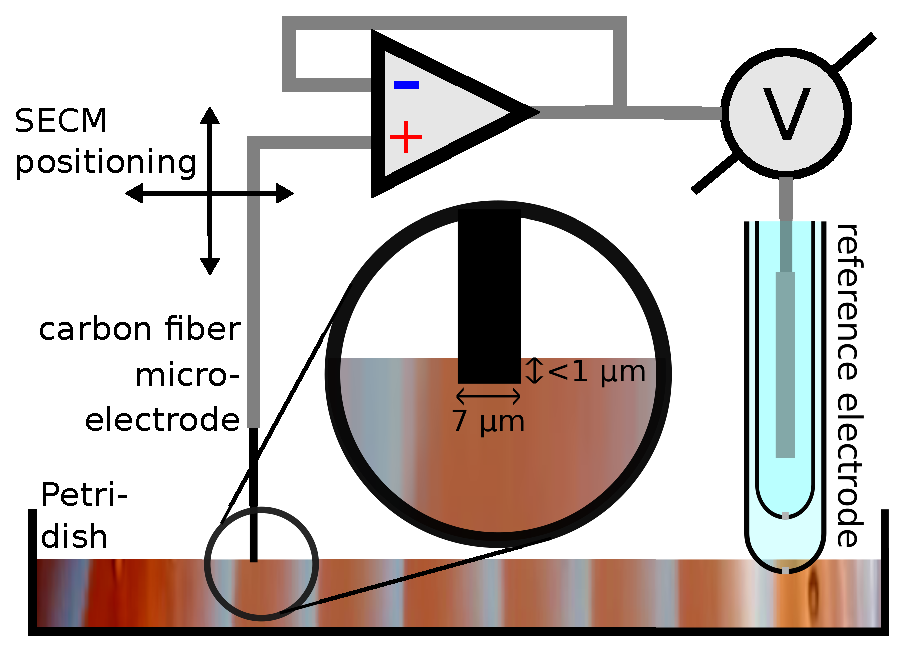
\includegraphics[width=0.45\textwidth]{setup.eps}

\begin{flushleft}
\textbf{B}
\end{flushleft}

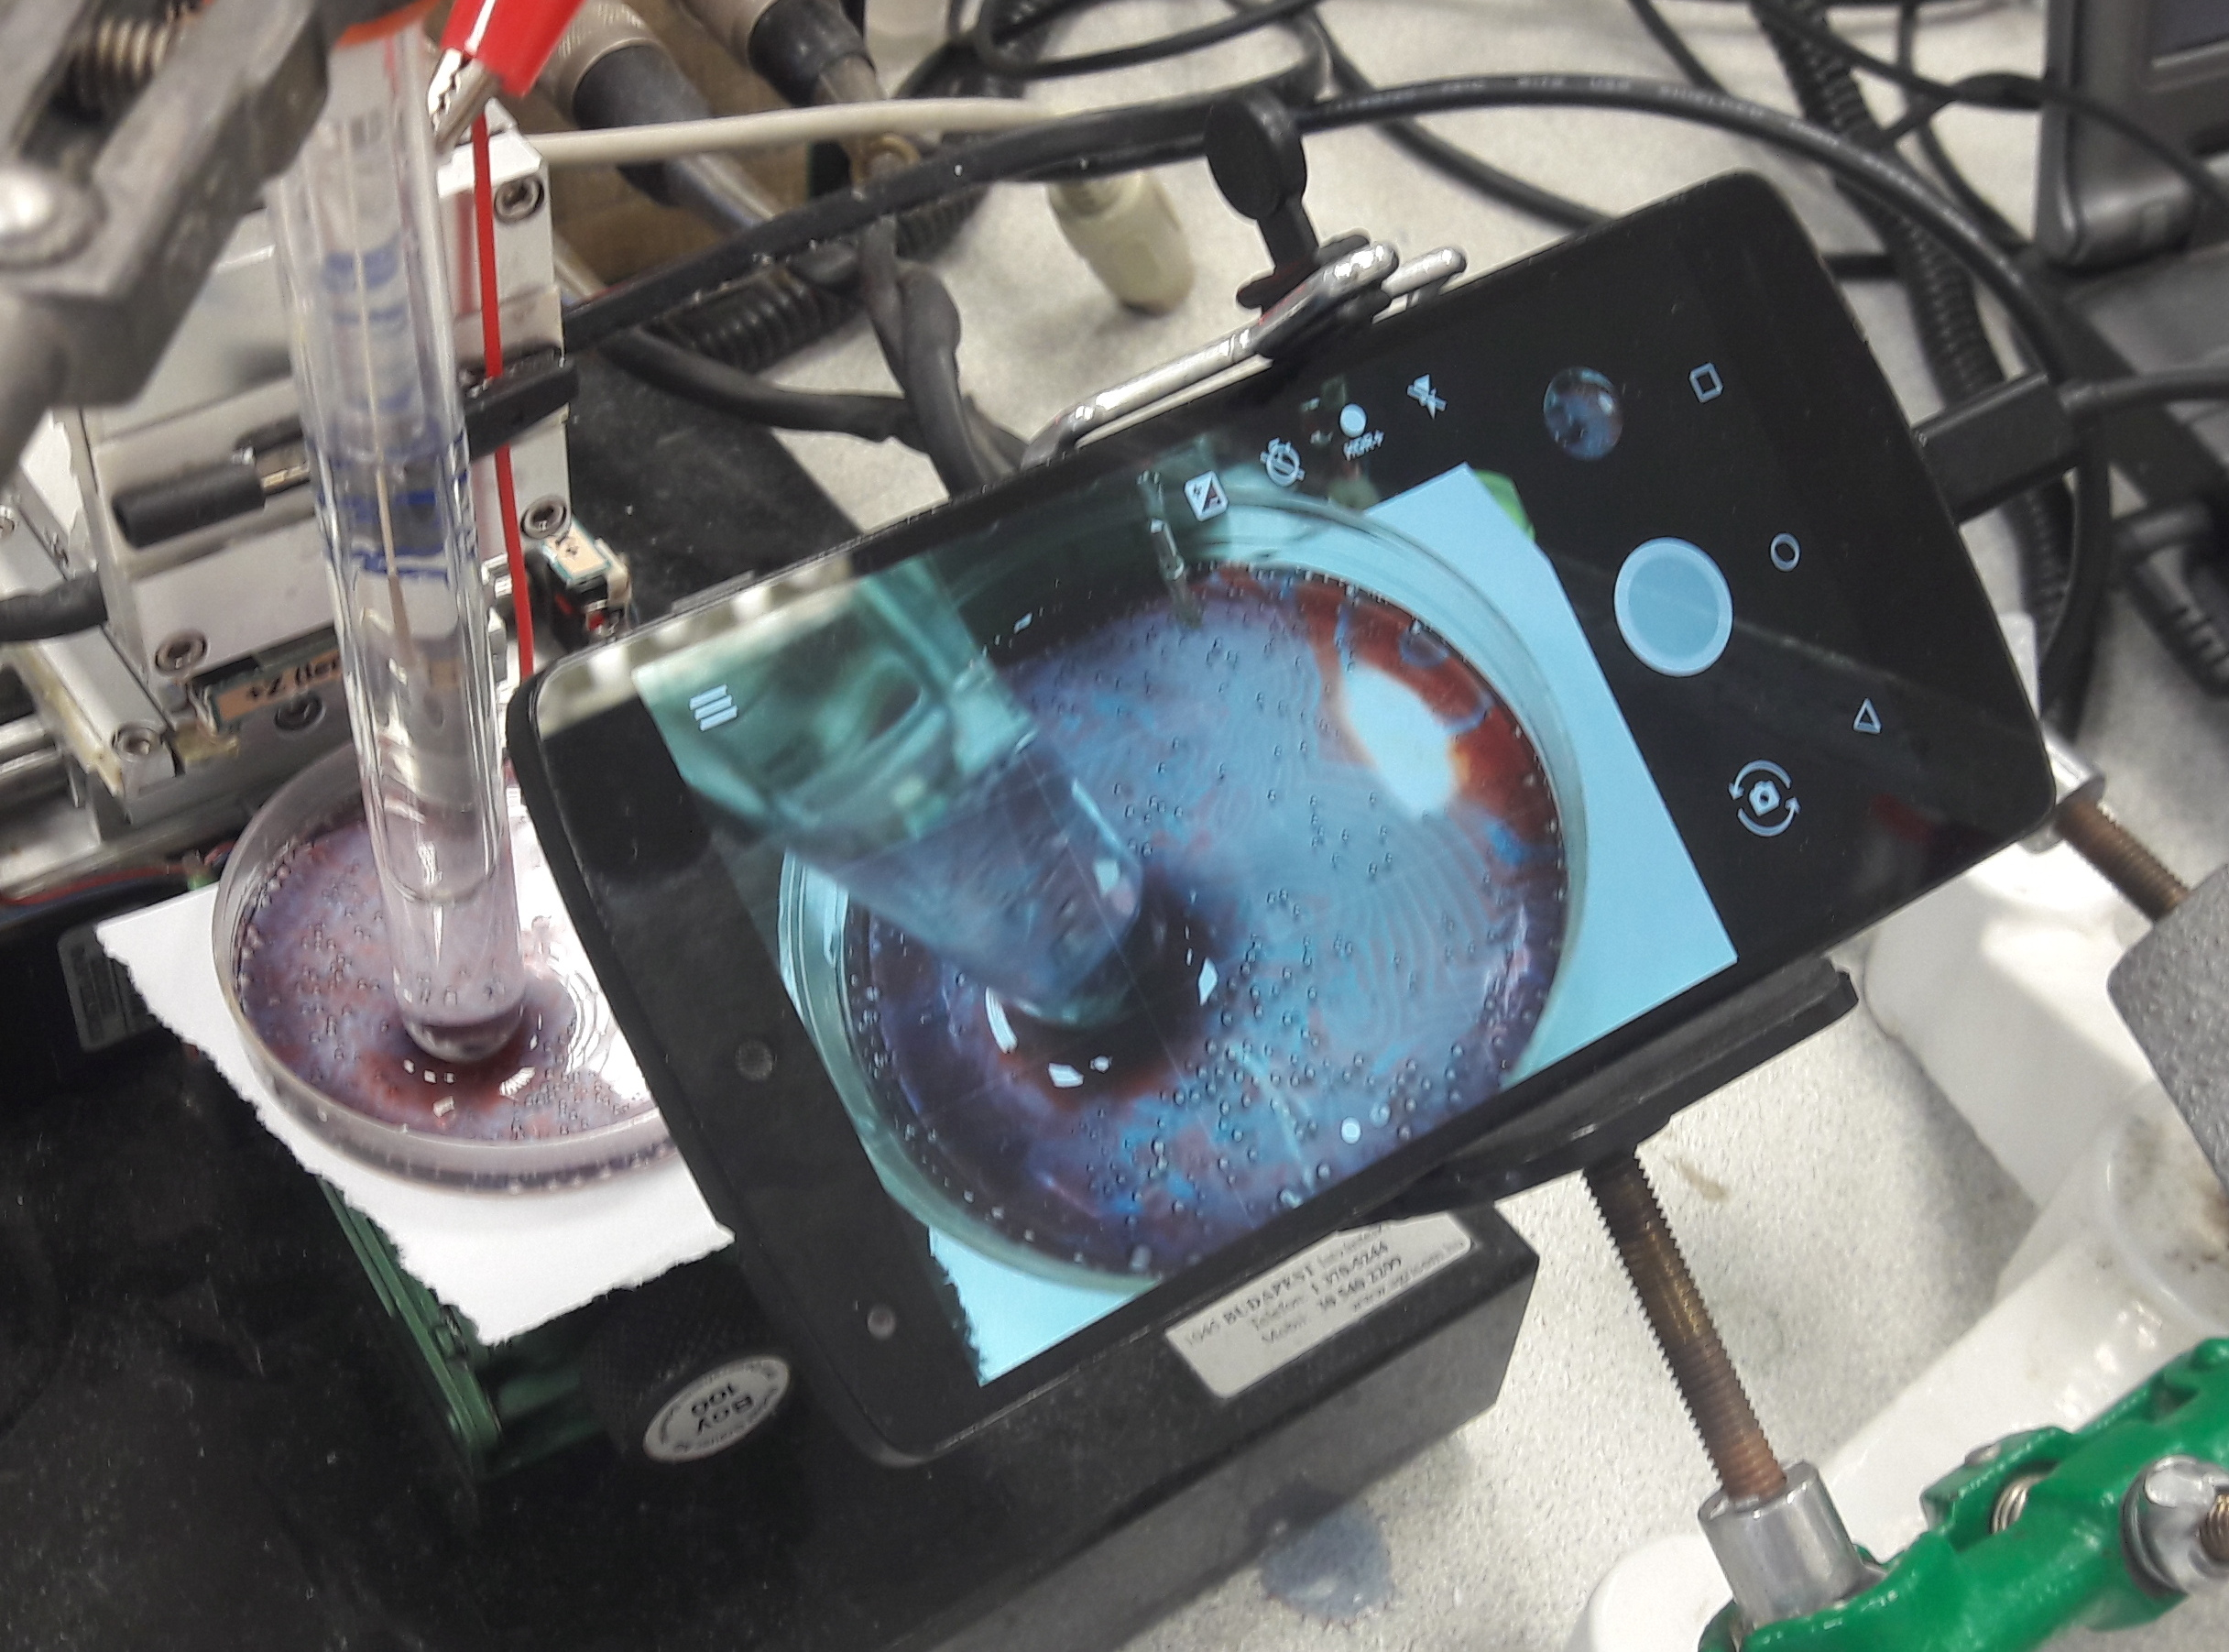
\includegraphics[width=0.45\textwidth]{setup_photo.jpg}

\begin{flushleft}
\textbf{C}
\end{flushleft}

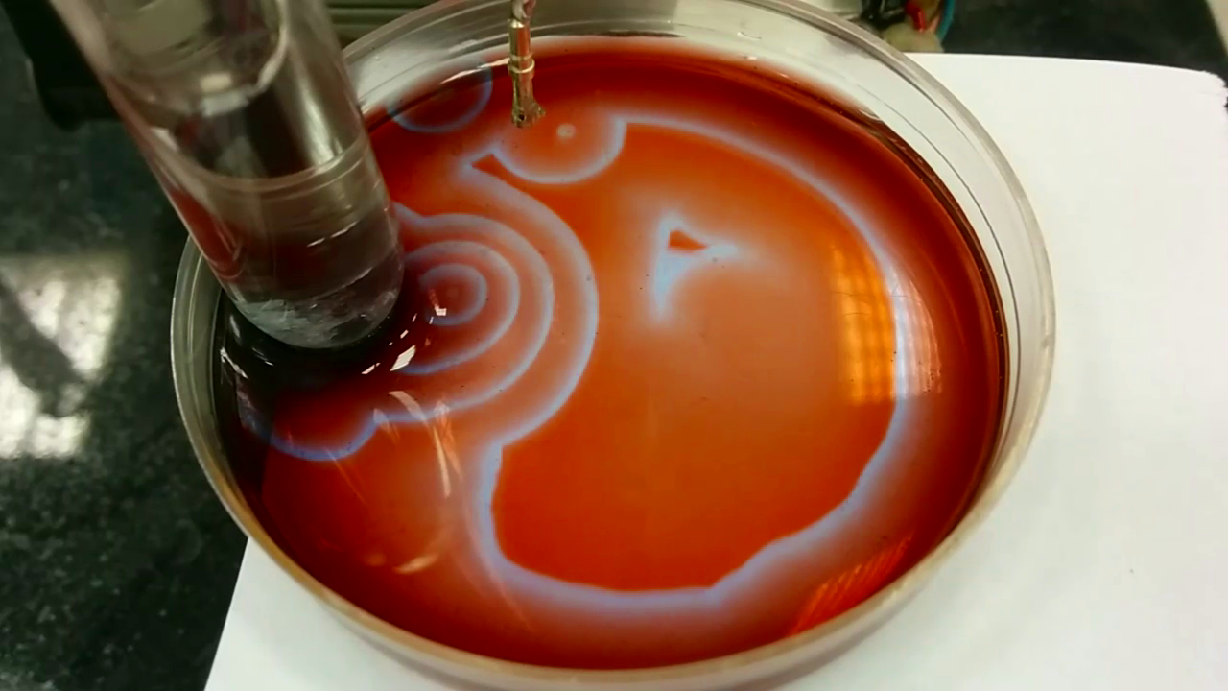
\includegraphics[width=0.45\textwidth]{0.png}

\caption{
Sketch (A) and photograph (B) of the experimental setup. (C) The image seen by the camera.
}
\label{fig:setup}
\end{figure}

\paragraph{Optical observation}
The reaction was filmed using an 8 MP Sony Exmor IMX179 1/3.2-inch CMOS sensor (as part of an LG Nexus 5 cell phone), positioned 10 cm from the scanline at a 45 degree angle, with the frame parallel to the scanline.
The space-time plot was prepared using the Blender 2.78 video editing software by grabbing linear, 1 pixel high images from every 30th frame of the video (1 s interval).
The position and orientation of these 1 pixel high frames matched that of the scanline covered by the microelectrode.
The image sequence was assambled by stacking the grabs vertically using Imagemagick 1.3.20.
The overlayed optical--electrochemical plot was created in Gnuplot 4.6.6.

\section{Results and discussion}

The experimental setup allowed several simplifications to be made. To minimize the convective effect of the indicator redox--electrode, only a very small, less than 1 $\upmu$m  portion of it was immersed in the reaction mixture. This in turn, allowed the use of an uninsulated electrode, because the sensitive area of the electrode was already limited a very small point. Without insulation, the electrode could be made even smaller. Another advantage of the setup is the perfectly smooth, flat and levelled surface of the liquid phase. Only the X--Y plane of the SECM had to be levelled. The thickness of the reaction mixture had to be minimized to be quasy--2D to allow the simultaneous recording of the optical space--time plot, which didn't make the SECM measurement any more difficult, since the tip was already being rastered on the surface of the reaction mixture. 

Fig. \ref{fig:spatiotemporal}A shows the electrochemical spatiotemporal image overlayed on top of the optical one.
The optical space--time plot is presented in grayscale to allow better visibility.
Lighter shade of gray means a higher ferriin/ferroin  ratio.
The measured redox potential represents the [Fe$^{2+}$]/[Fe$^{3+}$]  concentration ratio in the reaction, a relationship that is described by the Nernst-equation:

\begin{equation}
	E = E^\theta - \frac{RT}{F}\ln \frac{[Fe^{2+}]}{[Fe^{3+}]}
\end{equation}

The measured potential is certainly a mixed potential depending on several other species in the reaction, with the two largest contributors being the iron catalyst and bromate \cite{field1972oscillations}.
Despite this, a very good correlation can be observed between the changes of the potential of the carbon fiber microelectrode and the propagation of the oxidizing chemical waves that is visible in the optical image.
Fig. \ref{fig:grabs2}. shows the encounter of the moving microelectrode with wave \#3.
There is no evidence of any convective disturbance caused by the movement of the microelectrode.
This is important, because the BZ reaction is very sensitive to external influences, and it wouldn't be possible to properly observe it with a technique that significantly influences the reaction.
The 7 $\upmu$m microelectrode diameter is small enough that the convective effect is alleviated by diffusion to such an extent, that the reaction behaves as if the microelectrode wasn't there.

Parameters that can be determined from the optical data -- such as the travel speed of chemical waves -- can also be calculated from the SECM spatiotemporal measurements.
In case of stationary microelectrode, two of them would be necessary at a known distance from each other to calculate the travel speed.
It could be calculated as the ratio of the distance between the electrodes, and the time it takes for the wave to get from the first microelectrode to the second.
However, using the SECM, one microelectrode is sufficient because the tip can be repositioned to allow additional measurements of the same wave.
For instance, wave \#3 was encountered by the carbon microelectrode three times, at t$_1$=47 s, t$_2$=67 s and t$_3$=80 s.
The positions of these encounteres are also known: x$_1$=1400 $\upmu$m, x$_2$=6400 $\upmu$m and x$_3$=8600 $\upmu$m.
Based on these coordinates, the average travel speed of wave \#3 during its path between the two outermost positions is 218.18 $\upmu$m/s.
This value is comparable to the travelling speed of chemical waves reported by R. J. Field and R. M. Noyes \cite{field1974oscillationsV}, under slightly lower H$_2$SO$_4$ concentarions but otherwise similar initial reactant concentrations (4 -- 9 mm/min or 66.67 -- 150 $\upmu$m/s).
Table \ref{table:stats}. contains several parameters of the waves that were encountered multiple times by the microelectrode. 

\begin{table}
\caption{Chemical wave encounters by the microelectrode during the scanning process.}
\small
\label{table:stats}
\centering
\begin{tabular}{r c c c c c}
Wave \# & t, s & E, mV & x, mm & v, $\upmu$m/s \\
 \hline
 \hline
 3&\begin{tabular}{c}47\\67\\80\end{tabular}&\begin{tabular}{c}957\\978\\977\end{tabular}&\begin{tabular}{c}1.4\\6.4\\8.6\end{tabular}&218.8\\
 \hline
 6&\begin{tabular}{c}99\\114\\133.5\end{tabular}&\begin{tabular}{c}968\\975\\1027\end{tabular}&\begin{tabular}{c}1\\4.8\\7.6\end{tabular}&191.3\\
 \hline
 7&\begin{tabular}{c}148.5\\171\\181.5\end{tabular}&\begin{tabular}{c}1052\\1127\\1059\end{tabular}&\begin{tabular}{c}1.6\\7.2\\8.8\end{tabular}&218.18\\
 \hline
 9&\begin{tabular}{c}200\\219.5\\234.5\end{tabular}&\begin{tabular}{c}1016\\1074\\1016\end{tabular}&\begin{tabular}{c}1.4\\6.2\\8\end{tabular}&191.3\\
 \hline
 12&\begin{tabular}{c}253.5\\268\\287\end{tabular}&\begin{tabular}{c}1060\\1120\\1053\end{tabular}&\begin{tabular}{c}0.4\\5.2\\7.4\end{tabular}&208.96\\
\end{tabular}
\end{table}

Using only one electrode has additional advantages over using an array, for instance one doesn't have to worry about the differences between the electrodes.
Furthermore, when using an SECM in such study, the microelectrode can be positioned to any coordinate within the mechanical boundaries of the instrument.

One drawback is that the electrochemical information presented in Fig. \ref{fig:spatiotemporal}. is rather sparse compared to the optical image beneath.
An obvious improvement would be increasing the scanning speed, to make the scanlines more dense.
This is currently a limitation of the SECM instrument in our laboratory, and is subject to a subsequent paper.

The travel speeds calculated are certainly not accurate, since in the measurement both the temporal ($\delta$t=0.5 s) and the spatial ($\delta$x=200 $\upmu$m) data is discrete, hence the equal values for waves \#3 -- \#7 and waves \#6 -- \#9.

It must be mentioned, that these travel speeds are not radial, but rather measured on a chord of the circular waves.
Knowing that the angle at which the reaction has been filmed is 45 degrees, after determining the angle between the radius and the chord, the actual travel speed can be obtained.

\def\s{0.5}
\begin{figure}
%% trim = top left bottom right
\centering
\flushleft{\textbf{\large{A}}}
\includegraphics[trim = 15mm 60mm 0mm 30mm, clip, width=\s\textwidth, angle=-90]{spacetime.eps}
\flushleft{\textbf{\large{B}}}
\begin{tikzpicture}
  \begin{axis}[width=7cm, height=5cm, xlabel={x / cm},ylabel={time / s},zlabel={E / V}, zmin=0.9]
    \addplot3[very thick, color=red] table {17101308_st_lines_back.txt};
    \addplot3[very thick, color=blue] table {17101308_st_lines_there.txt};
  \end{axis}
\end{tikzpicture}
\caption{(A) Electrochemical space-time plot overlayed on top of the corresponding optical one.
The potential of the carbon fiber microelectrode is shown as a function of spatiotemporal coordinates.
Redox indicator was ferroin.
The measured redox potential corresponds to the ferroin/ferriin ratio in the system.
The optical spatiotemporal image was grayscaled to allow better visibility when overlaying the electrochemical data.
The brighter stripes correspond to the oxidizing waves.
(B) The second scan cycle.
Blue line: forward scan, red line: backwards scan.
}
\label{fig:spatiotemporal}
\end{figure}

\begin{figure}
\centering
\begin{tikzpicture}
    \draw (0, 0) node[inner sep=0] {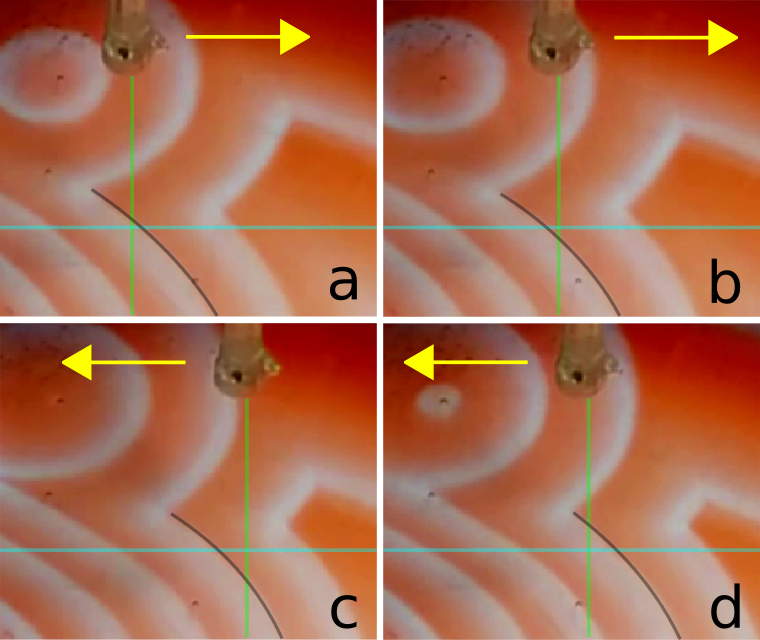
\includegraphics[width=0.45\textwidth]{grabs.png}};
\end{tikzpicture}
\caption{Frame grabs from the video that was recorded during the experiment.
Numbers represent the order of the chemical waves, same as in Fig. \ref{fig:spatiotemporal}.
(a)--(b) 2 seconds before and after the carbon fiber reaches wave \#3 while traveling in the same direction.
(c)--(d) 2 seconds before and after the carbon fiber reaches wave \#3 while traveling in the opposite direction.
Due to its small size, the carbon fiber itself, and the point where it touches the surface of the reaction mixture is invisible in these images.
The green -- vertical -- line reperesents the \emph{y}-coordinate of the point where the carbon fiber touches the surface.
The blue -- horizontal -- line marks the scanline.
Wave \#3 is marked by the black line.
The pin header that was holding the carbon fiber is visible in the top portion of the images.
}
\label{fig:grabs2}
\end{figure}

Fig. \ref{fig:spatiotemporal}B. shows the second scan cycle.
The forward and backward scans are similar, as an indication that the shape of the potential recording is independent of the scan direction.
Both curves have a sharp peak, making the determination of wavelength and period time easier, compared to curves derived from 2D optical measurements such as in \cite{muller1985structure} and \cite{nagy1990experimental}.
Another advantage of the potentiometric method is that it can reach a higher resolution than the optical methods.
Nanometer sized potentiometric microsensors are now routinely prepared \cite{elsamadisi2010polished}.
Efforts toward further miniaturization would make the potentiometric study of the BZ and other reaction-diffusion processes at the nano- and microscales more viable \cite{epstein2016reaction}.

\section{Conclusions}
Potentiometry has been used to study the BZ reaction almost since its discovery.
Compared to the optical methods, it allowed farther reaching conclusions to be made by several research groups.
There is however one area where electrochemical investigations certainly lacked; they couldn't provide spatial information, which 2D photometry or tomography could easily do.
In this paper, we made an attempt to combine the advantages of the two techniques.
In its current form the technique has several limitations, for instance, the relatively low density of the electrochemical data.
%Further development can be expected.

Using potentiometric SECM with a sufficiently small microelectrode, the redox potential can be spatially resolved in a quasy-2D BZ reaction, without influencing the reaction.
By substituting the indicator tip or combining multiple ones, other parameters can be measured, possibly simultaneously.
With an appropriately small ion-selective microelectrode, it would also be possible to map the bromide-ion activity in the BZ reaction.
There are several extensive works on the use of such ion-selective electrodes in the study of the stirred BZ and other oscillating reactions \cite{noszticzius1982use, noszticzius1983use}.
A pH-sensitive antimony microelectrode with a less than 7 $\upmu$m diameter can be easily prepared, and it also might be possible to map pH in pH-regulated oscillators \cite{orban2015ph} with the SECM.
%This could provide an opportunity to further advance our understanding of the BZ and other oscillating reactions.

\section*{Acknowledgements}
The work was financially supported by the National Research, Development and Innovation Office (Budapest, Hungary) under grant K125244.
%András Kiss is thankful for the inspiring discussions with Gyula Hoffmann about pattern formation.

\bibliography{bz}{}
\bibliographystyle{unsrt}

\end{document}
